\section{Architecture of the System}
\phantomsection
\subsection{UML Diagrams}
The Unified Modeling Language (UML)\cite{uml} is a development and all use modeling language in the field of software engineering. Is indended to assure a standard way of visualizing the design of the system that it was made for.
To describe Kyno, the following UML diagrams will be used
\begin{itemize}
\item Use Case Diagram;
\item Deployment Diagram;
\item Class Diagram
\item Sequence Diagram;
\item Activity Diagram;
\item State Diagram.

\end{itemize}
These diagrams will illustrate the users possibilities, the system architecture and will also illustrate the procedures of interaction between the modules.

\subsubsection{Use Case Diagram}
To model a system the most important aspect is to capture the dynamic behaviour. In UML there are five diagrams available to model dynamic nature and use case diagram is one of them. Now as we have to discuss that the use case diagram is dynamic in nature there should be some internal or external factors for making the interaction.

These internal and external agents are known as actors. So use case diagrams are consists of actors, use cases and their relationships. The diagram is used to model the system/subsystem of an application. A single use case diagram captures a particular functionality of a system.

So to model the entire system n numbers of use case diagrams are used.

Purpose of Use Case diagram is:

\begin{itemize}
\item Used to gather requirements of a system.
\item Identify external and internal factors influencing the system.
\item Show the interacting among the requirements are actors.
\item Used to get an outside view of a system.

\end{itemize}



In the \mbox{figure \ref{uc_general}} , is shown the process
\begin{figure}[!h]
\centering
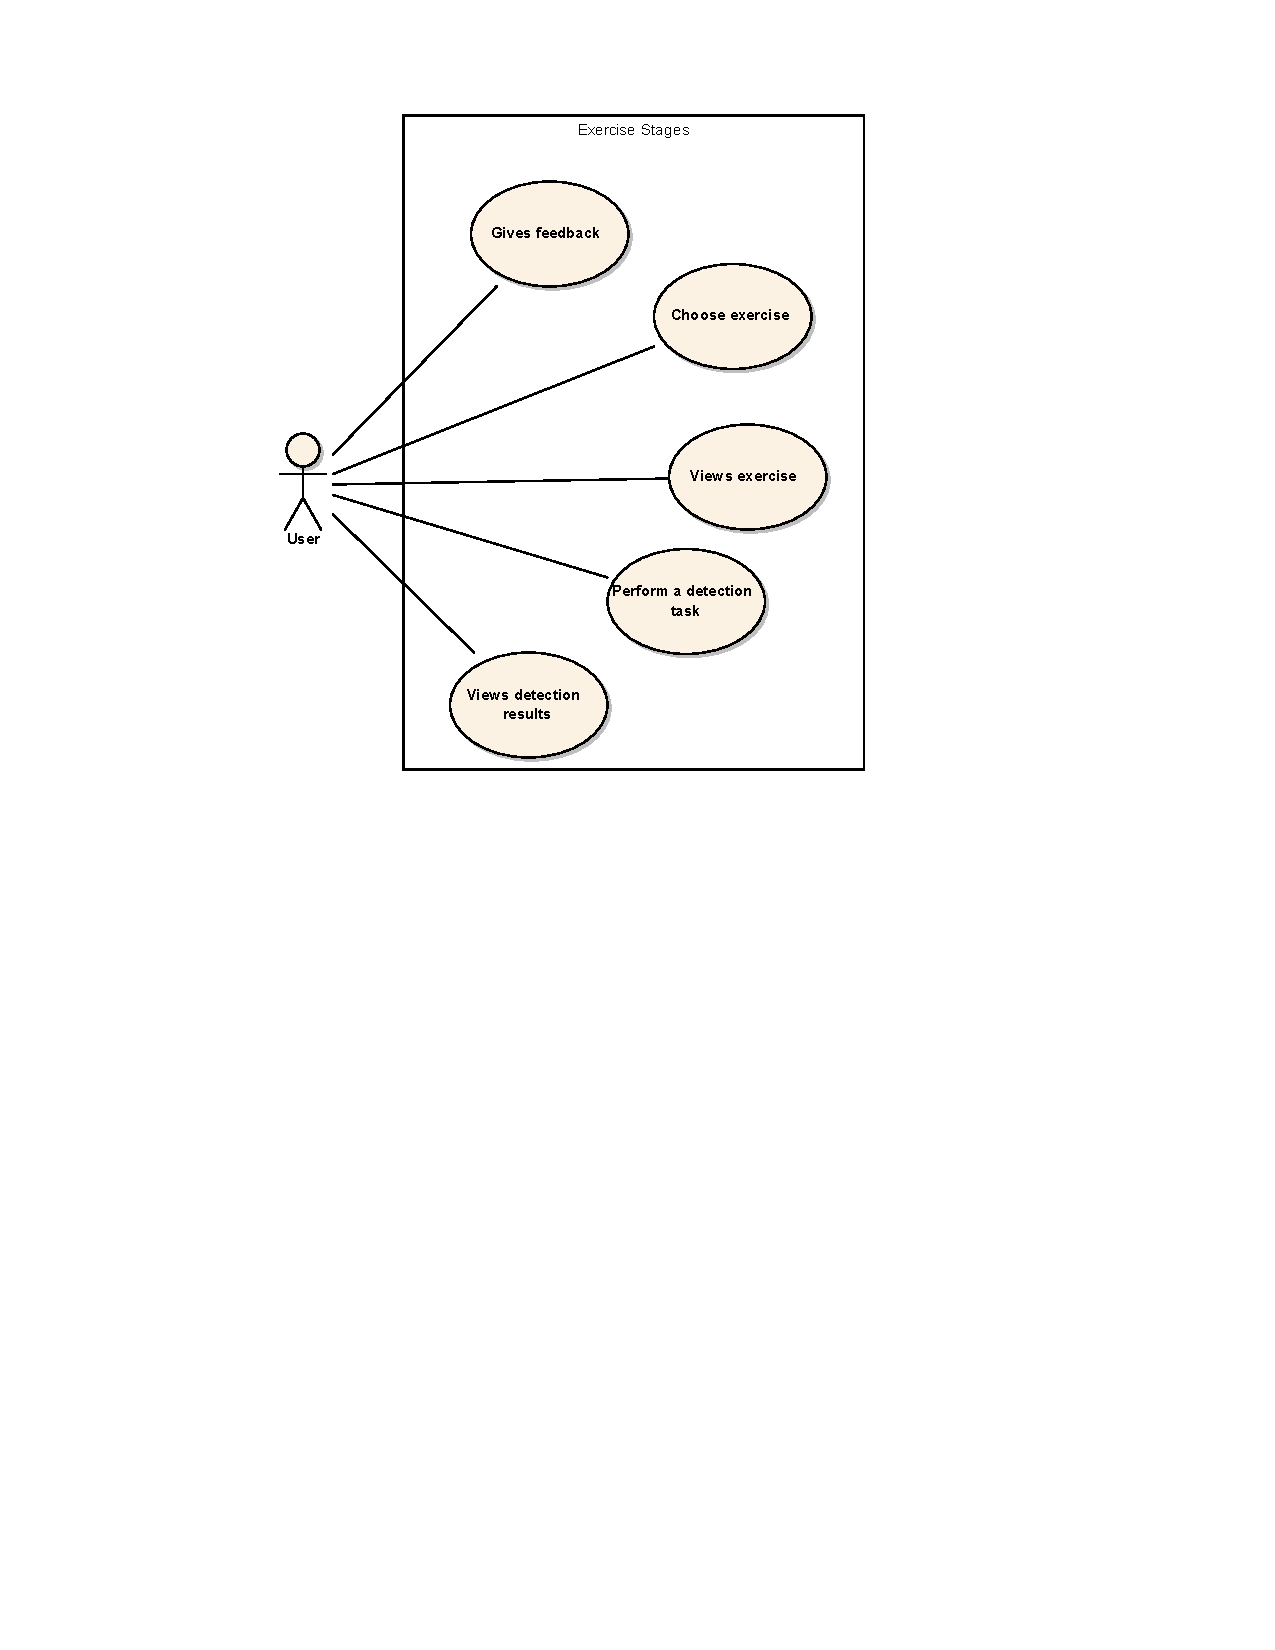
\includegraphics[trim={0 14.5cm 0 1cm},clip, width = 16cm]{2_uc_general}
\caption{General Use Case diagram of the system.}\label{uc_general}
\end{figure}

\begin{figure}[!h]
\centering
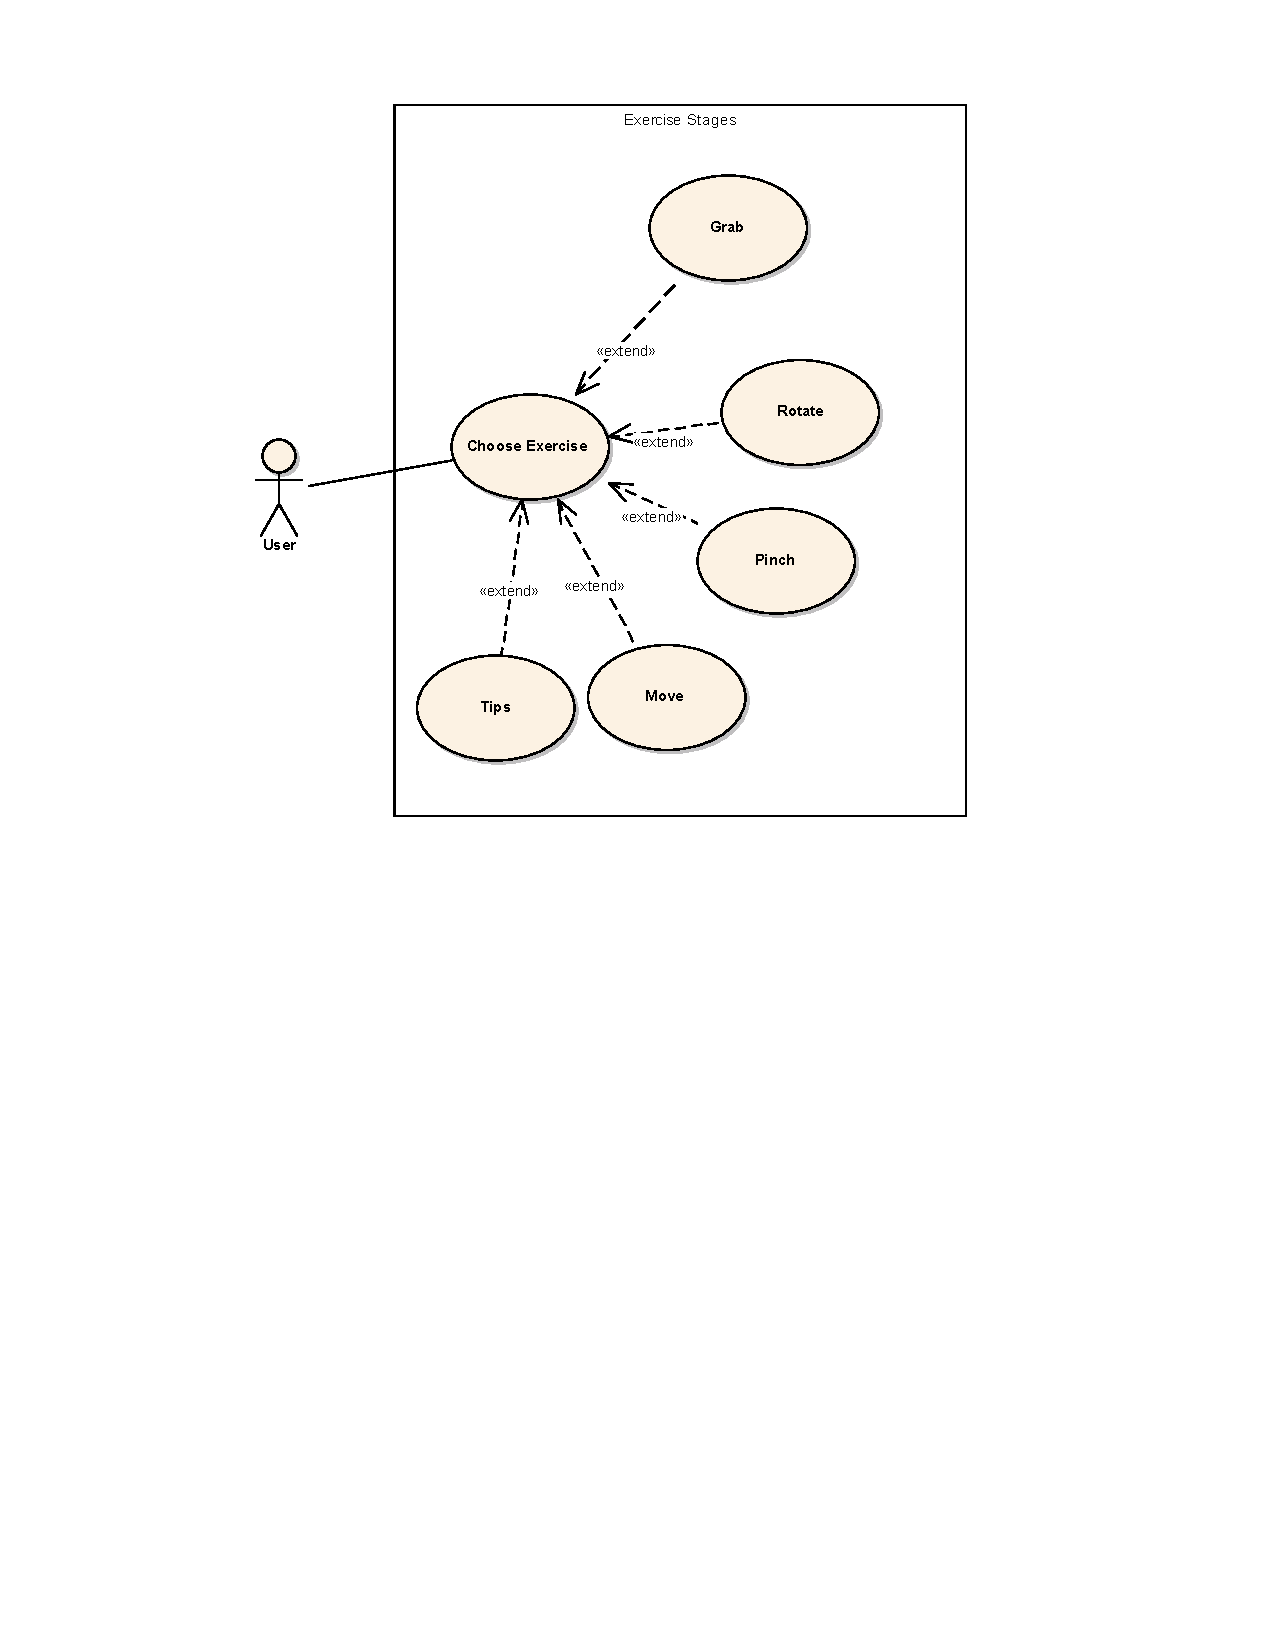
\includegraphics[trim={0 14cm 0 1cm},clip, width = 16cm]{1_uc_exercise_stage}
\caption{Use Case diagram of exercise steps.}\label{uc_exercise}
\end{figure}

\clearpage
\subsubsection{Deployment Diagram}
Deployment diagrams are used to visualize the topology of the physical components of a system where the software components are deployed.

So deployment diagrams are used to describe the static deployment view of a system. Deployment diagrams consist of nodes and their relationships.

The purpose of deployment diagrams can be described as:
\begin{itemize}
\item Describe runtime processing nodes.
\item Describe the hardware components used to deploy software components.
\item Visualize hardware topology of a system.
\end{itemize}




\begin{figure}[!h]
\centering
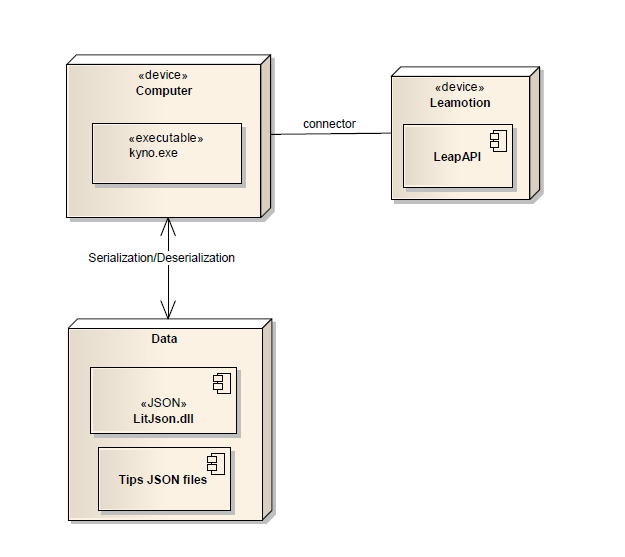
\includegraphics[trim={0 15.5cm 0 2cm},clip, width = 16cm]{1_deploy_diagram}
\caption{Deploy diagram of the system.}\label{deploy_diagram}
\end{figure}

\clearpage

\subsubsection{Class Diagram}
The class diagram is a static diagram and itrepresents the static view of an application. Describes the attributes and operations of a class and more than that, also the constraints appointed on the system.
Because class diagrams are the only UML diagrams that can be mapped directly with object oriented languages it is widely used in the modelling of the object oriented system and at the time of system construction.

Purpose of the class diagram can be summarized in:

\begin{itemize}
\item Analysis and design of the static view of an application.
\item Describe responsibilities of a system.
\item Base for component and deployment diagrams.
\item Forward and reverse engineering.
\end{itemize}




\begin{figure}[!h]
\centering
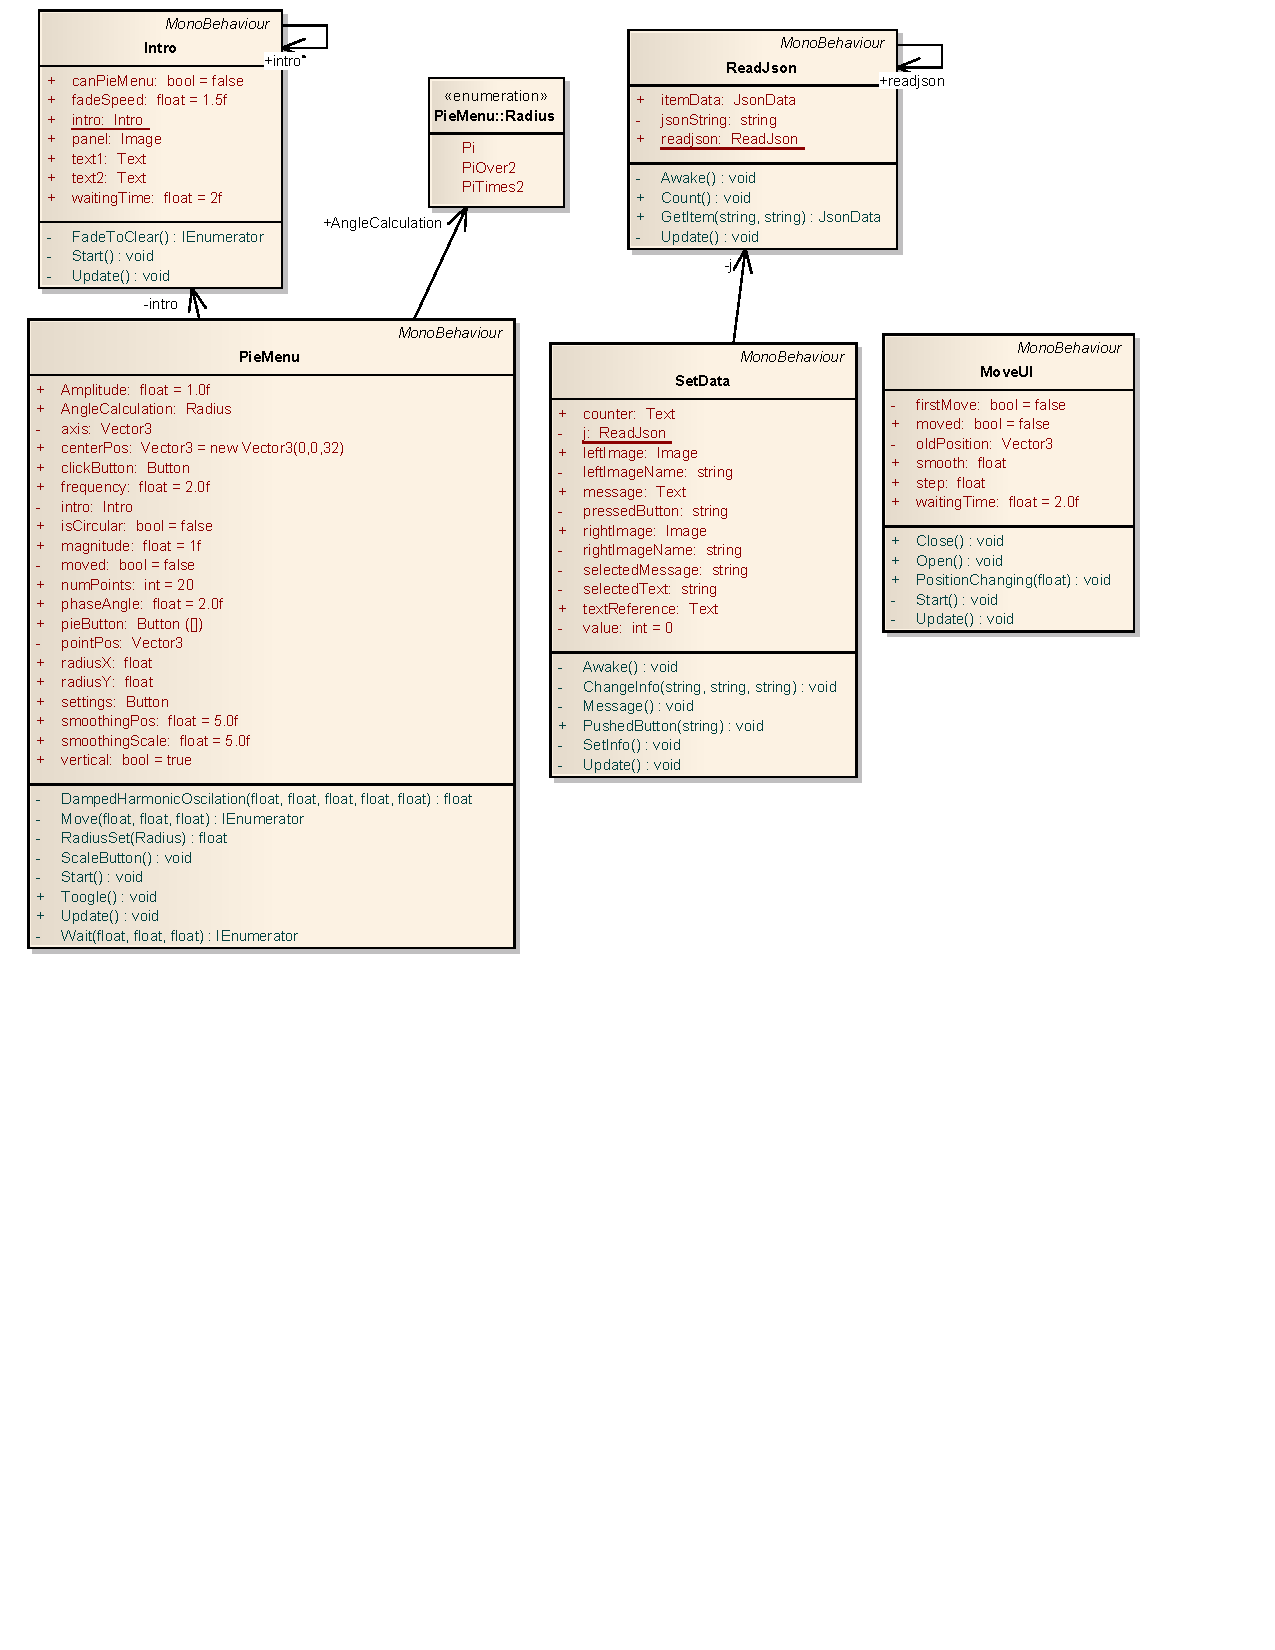
\includegraphics[trim={0 11cm 0 0cm},clip, width=16cm]{1_class_ui}
\caption{Class Diagram of User Interface and User Interaction.}\label{class_ui}
\end{figure}

\clearpage

\begin{figure}[!h]
\centering
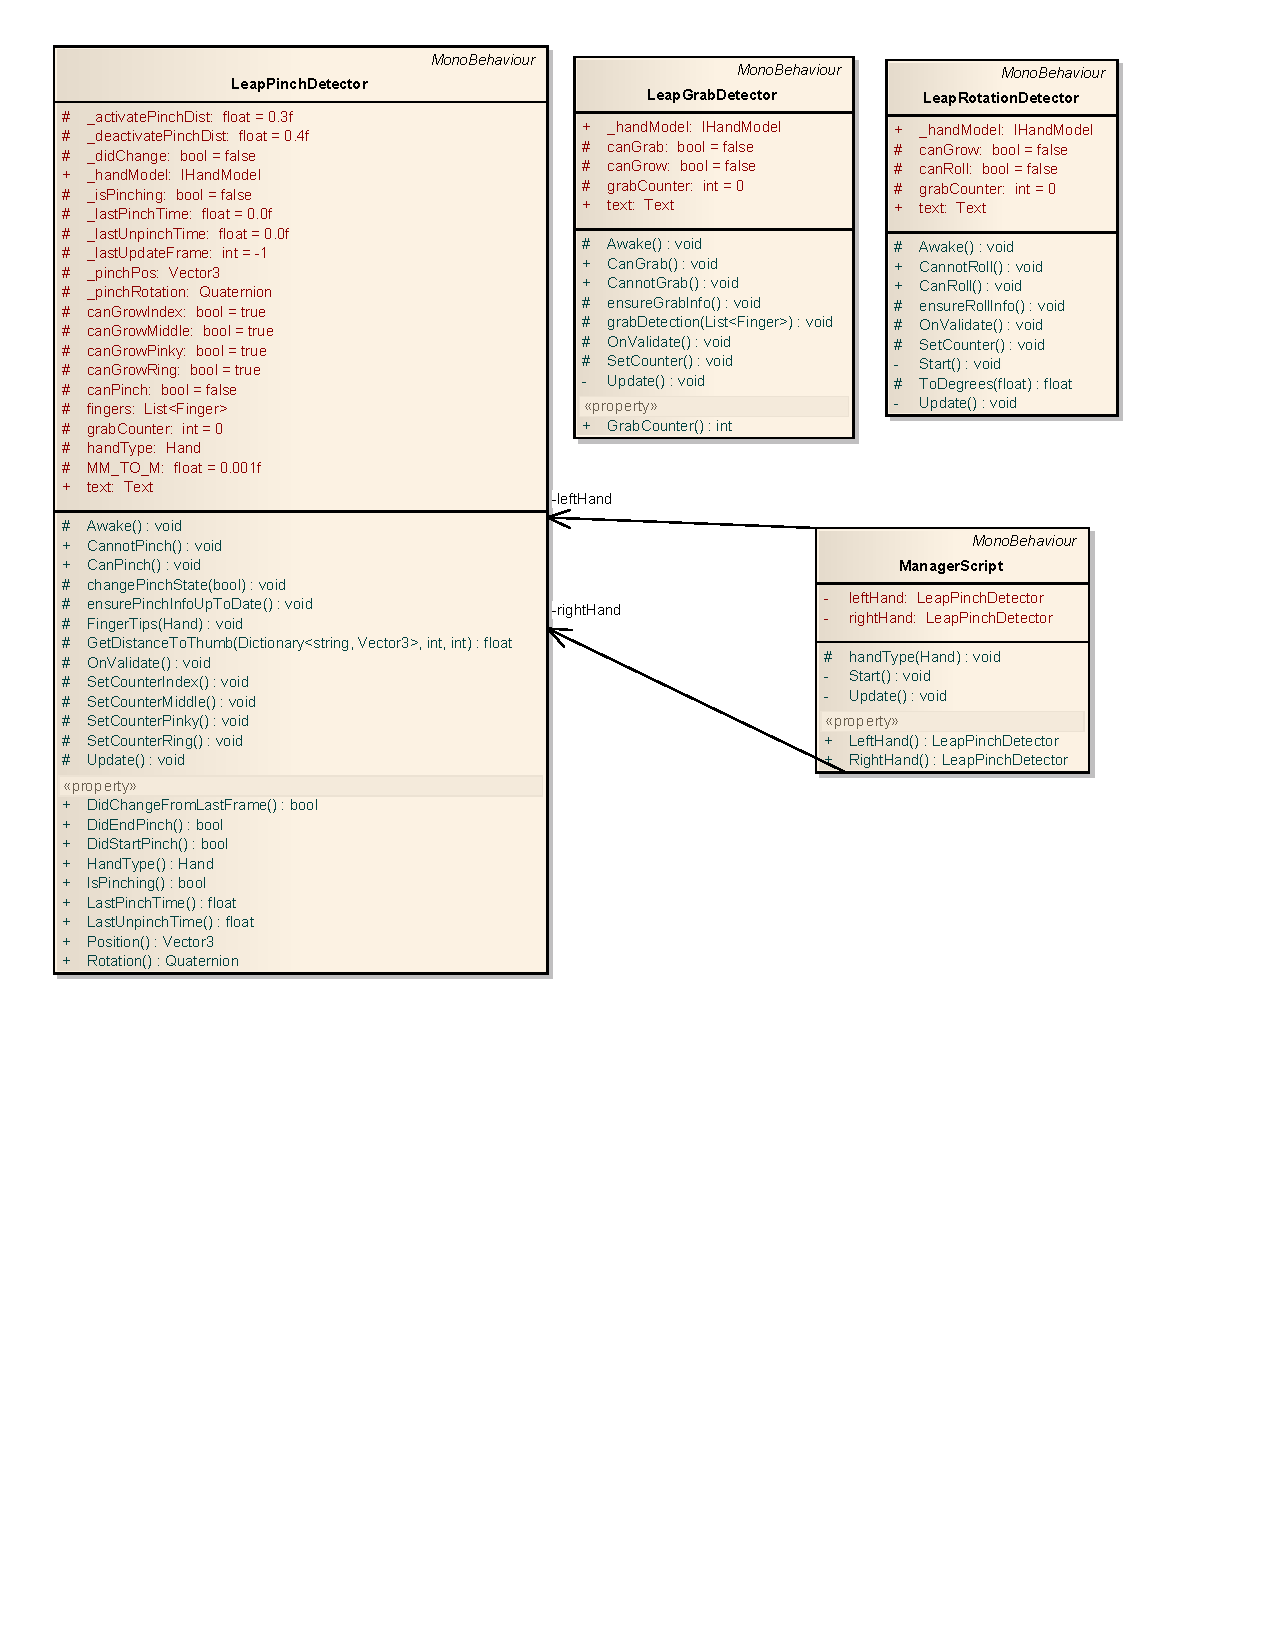
\includegraphics[trim={0 11cm 0 0.5cm},clip, width=16cm]{2_class_leapstates}
\caption{Class Diagram of Leap Motion gesture tracking.}\label{class_leap}
\end{figure}

\clearpage

\subsubsection{Sequence Diagram}
\begin{figure}[!h]
\centering
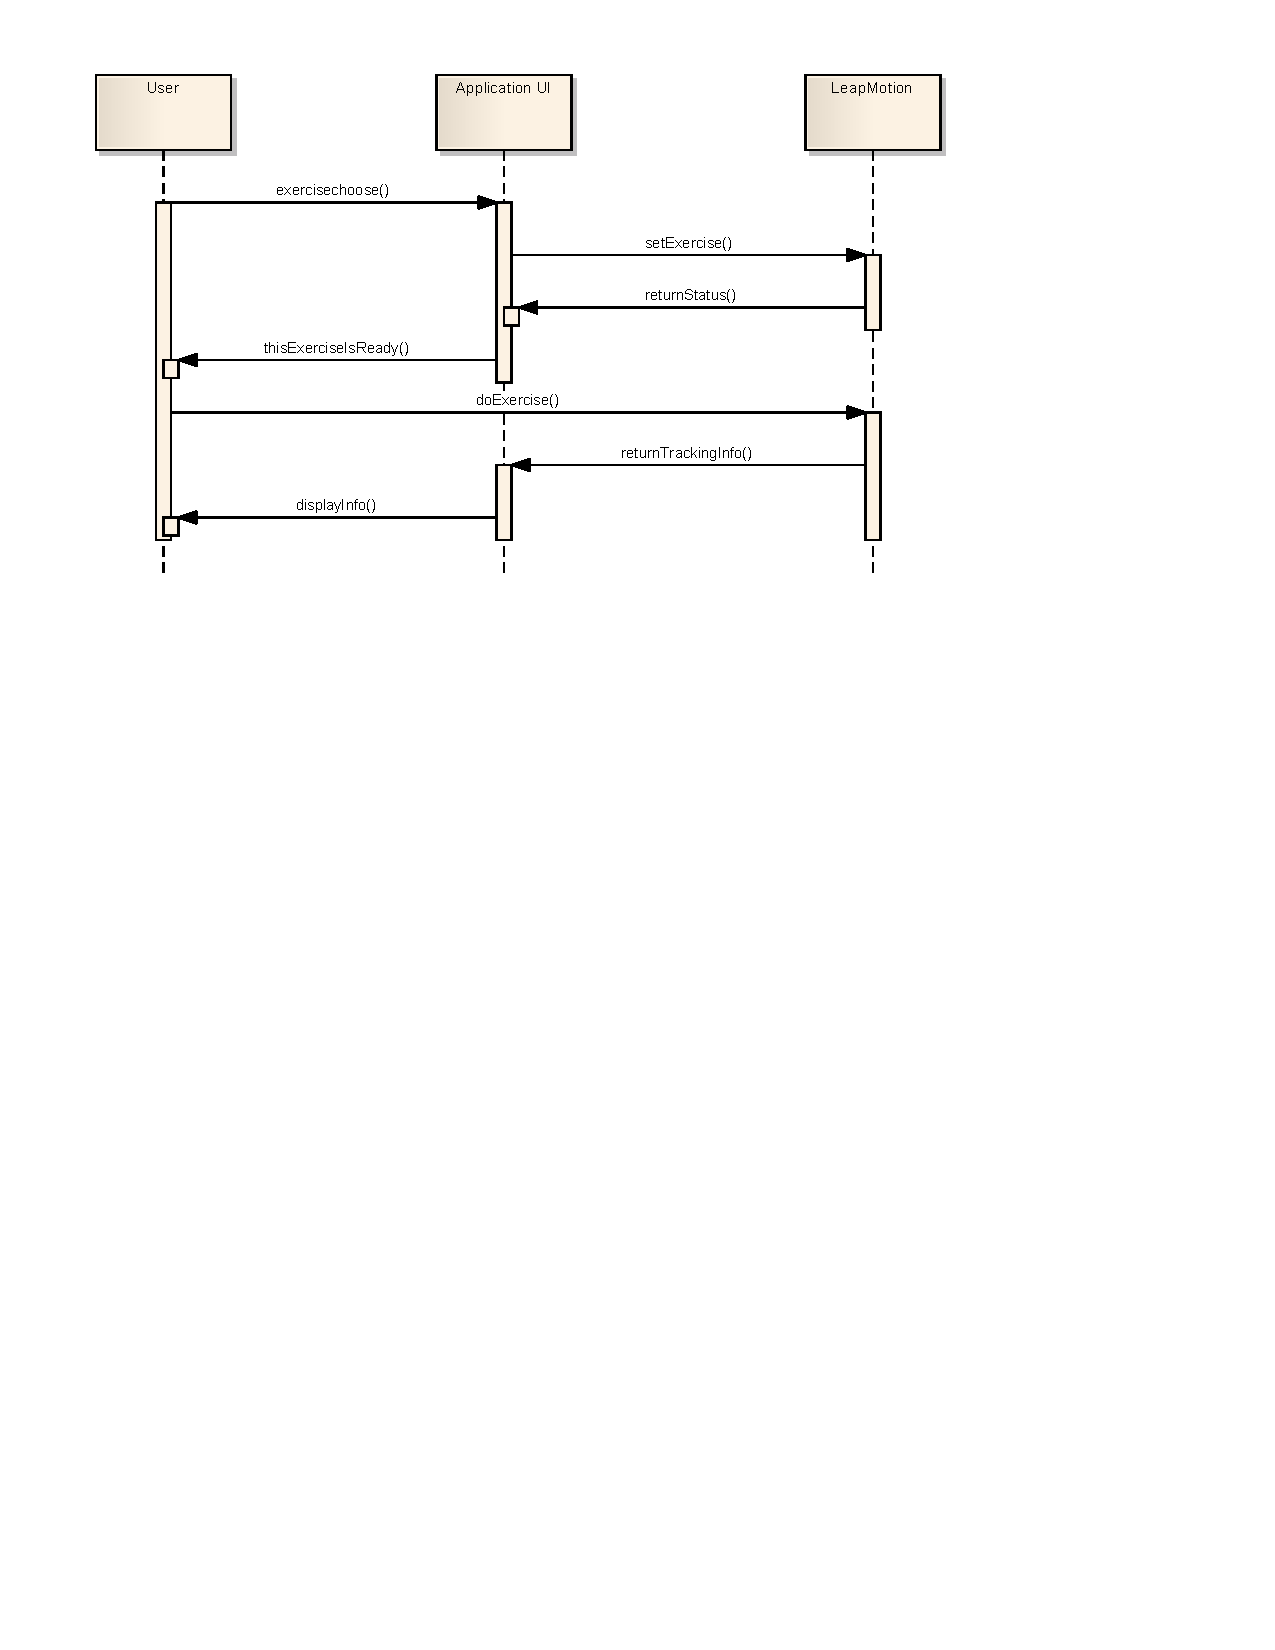
\includegraphics[trim={0 18cm 0 1cm},clip, width = 16cm]{1_sequence_exercise}
\caption{Sequence diagram of doing an exercise set.}\label{sequence_exercise}
\end{figure}

\clearpage

\subsubsection{Activity Diagram}
Activity diagram is another important diagram in UML to describe dynamic aspects of the system. This diagram is basically a flow chart to represent the flow form one activity to another activity. The activity can be described as an operation of the system.

So the control flow is drawn from one operation to another. This flow can be sequential, branched or concurrent. Activity diagrams deals with all type of flow control by using different elements like fork, join etc.


Purpose of activity diagram can be:
\begin{itemize}
\item Draw the activity flow of a system.
\item Describe the sequence from one activity to another.
\item Describe the parallel, branched and concurrent flow of the system.
\end{itemize}





\begin{figure}[!h]
\centering
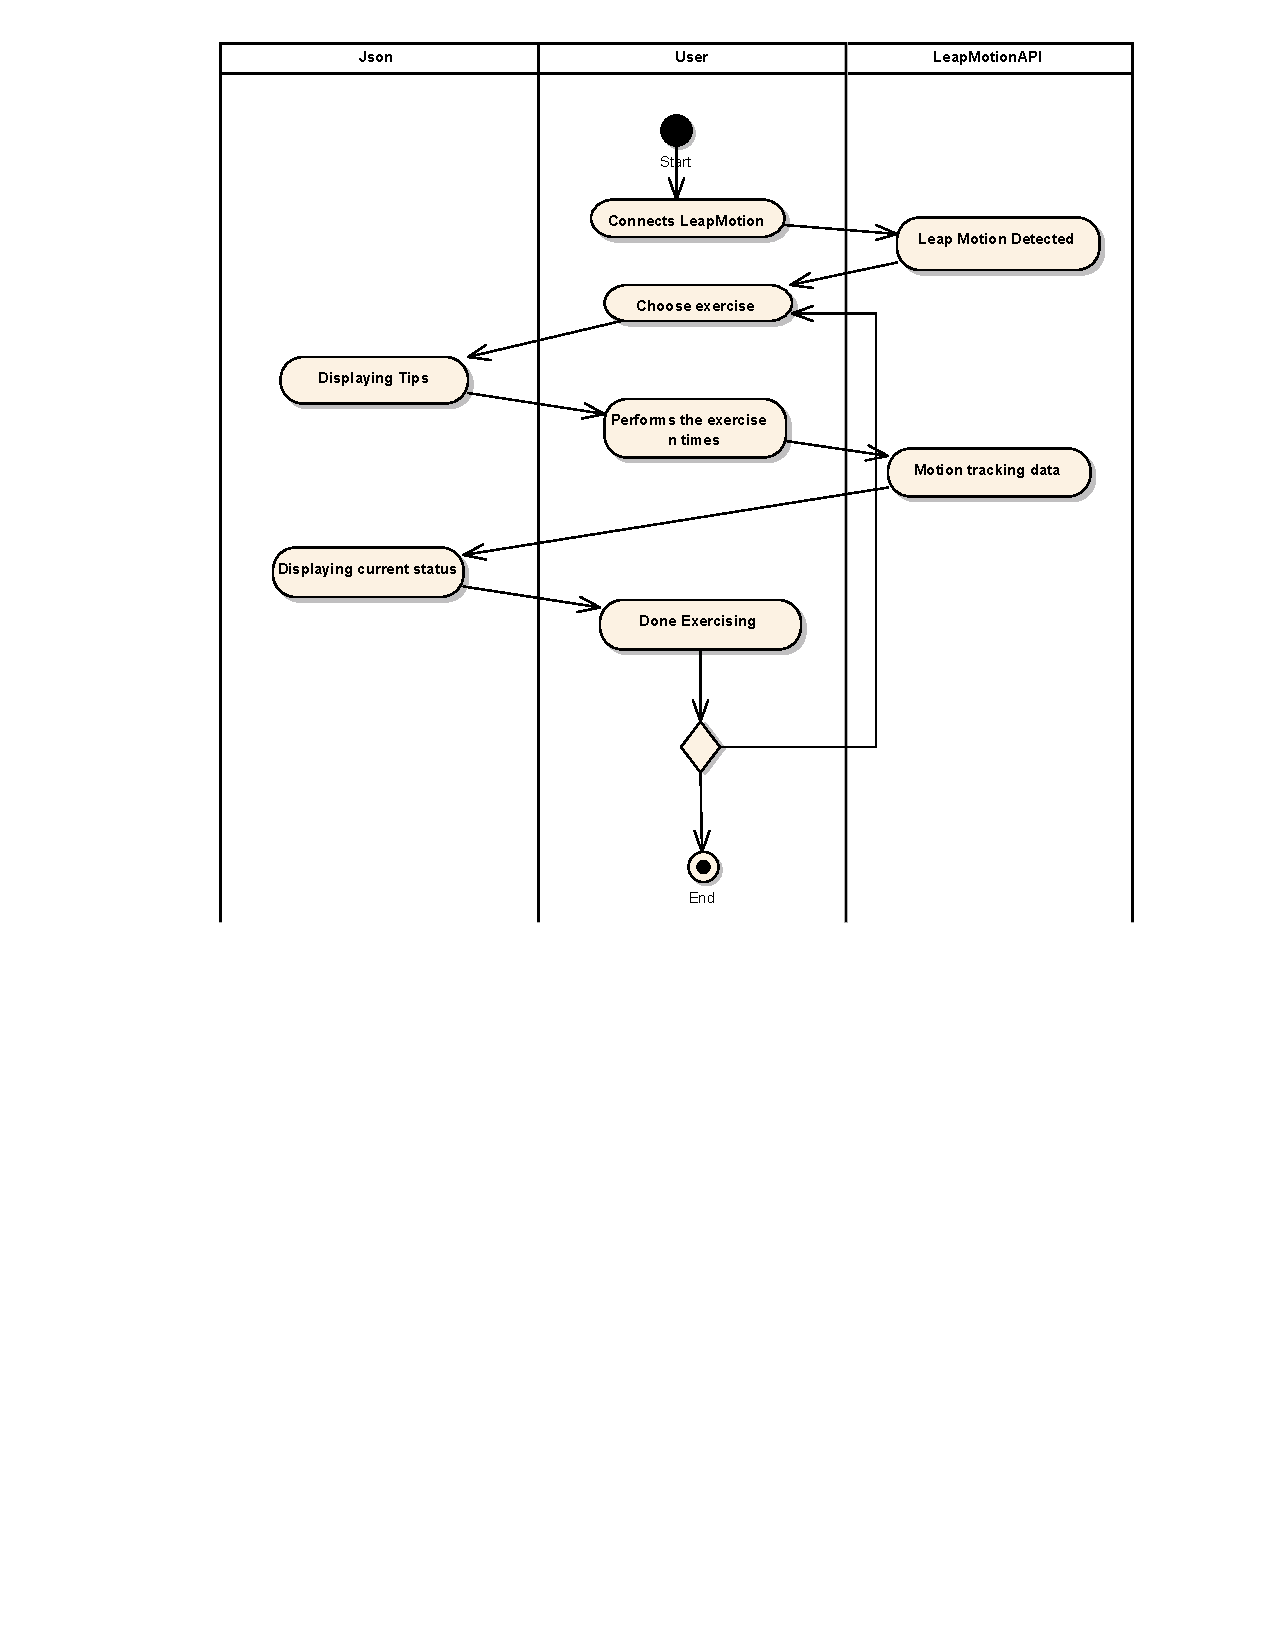
\includegraphics[trim={2cm 14cm 0 0.5cm},clip, width = 16cm]{1_activity_performs_exercise}
\caption{Activity diagram of performing an exercise.}\label{activity_performs}
\end{figure}

\clearpage

\subsubsection{State Diagram}
The name of the diagram itself clarifies the purpose of the diagram and other details. It describes different states of a component in a system. The states are specific to a component/object of a system.

A Statechart diagram describes a state machine. Now to clarify it state machine can be defined as a machine which defines different states of an object and these states are controlled by external or internal events.

Statechart diagrams are also used for forward and reverse engineering of a system. But the main purpose is to model reactive system.


Following are the main purposes of using Statechart diagrams:

\begin{itemize}
\item Define a state machine to model states of an object.
\item To model life time of a reactive system.
\item To model dynamic aspect of a system.
\item To describe different states of an object during its life time.
\end{itemize}







\begin{figure}[!h]
\centering
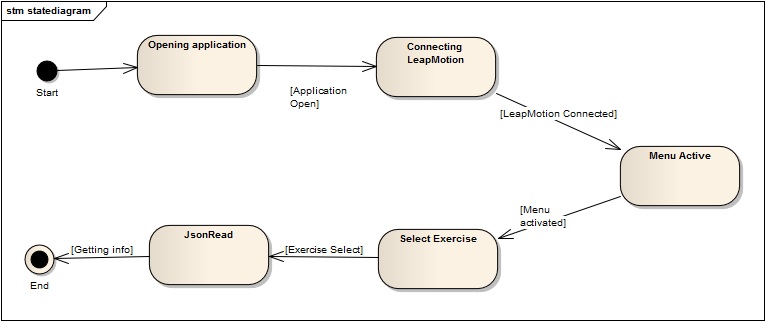
\includegraphics[trim={0 18cm 0 2cm},clip, width = 16cm]{1_state_chooseExercise}
\caption{Activity diagram of choosing and exercise.}\label{state_choose}
\end{figure}

\clearpage

\begin{figure}[!h]
\centering
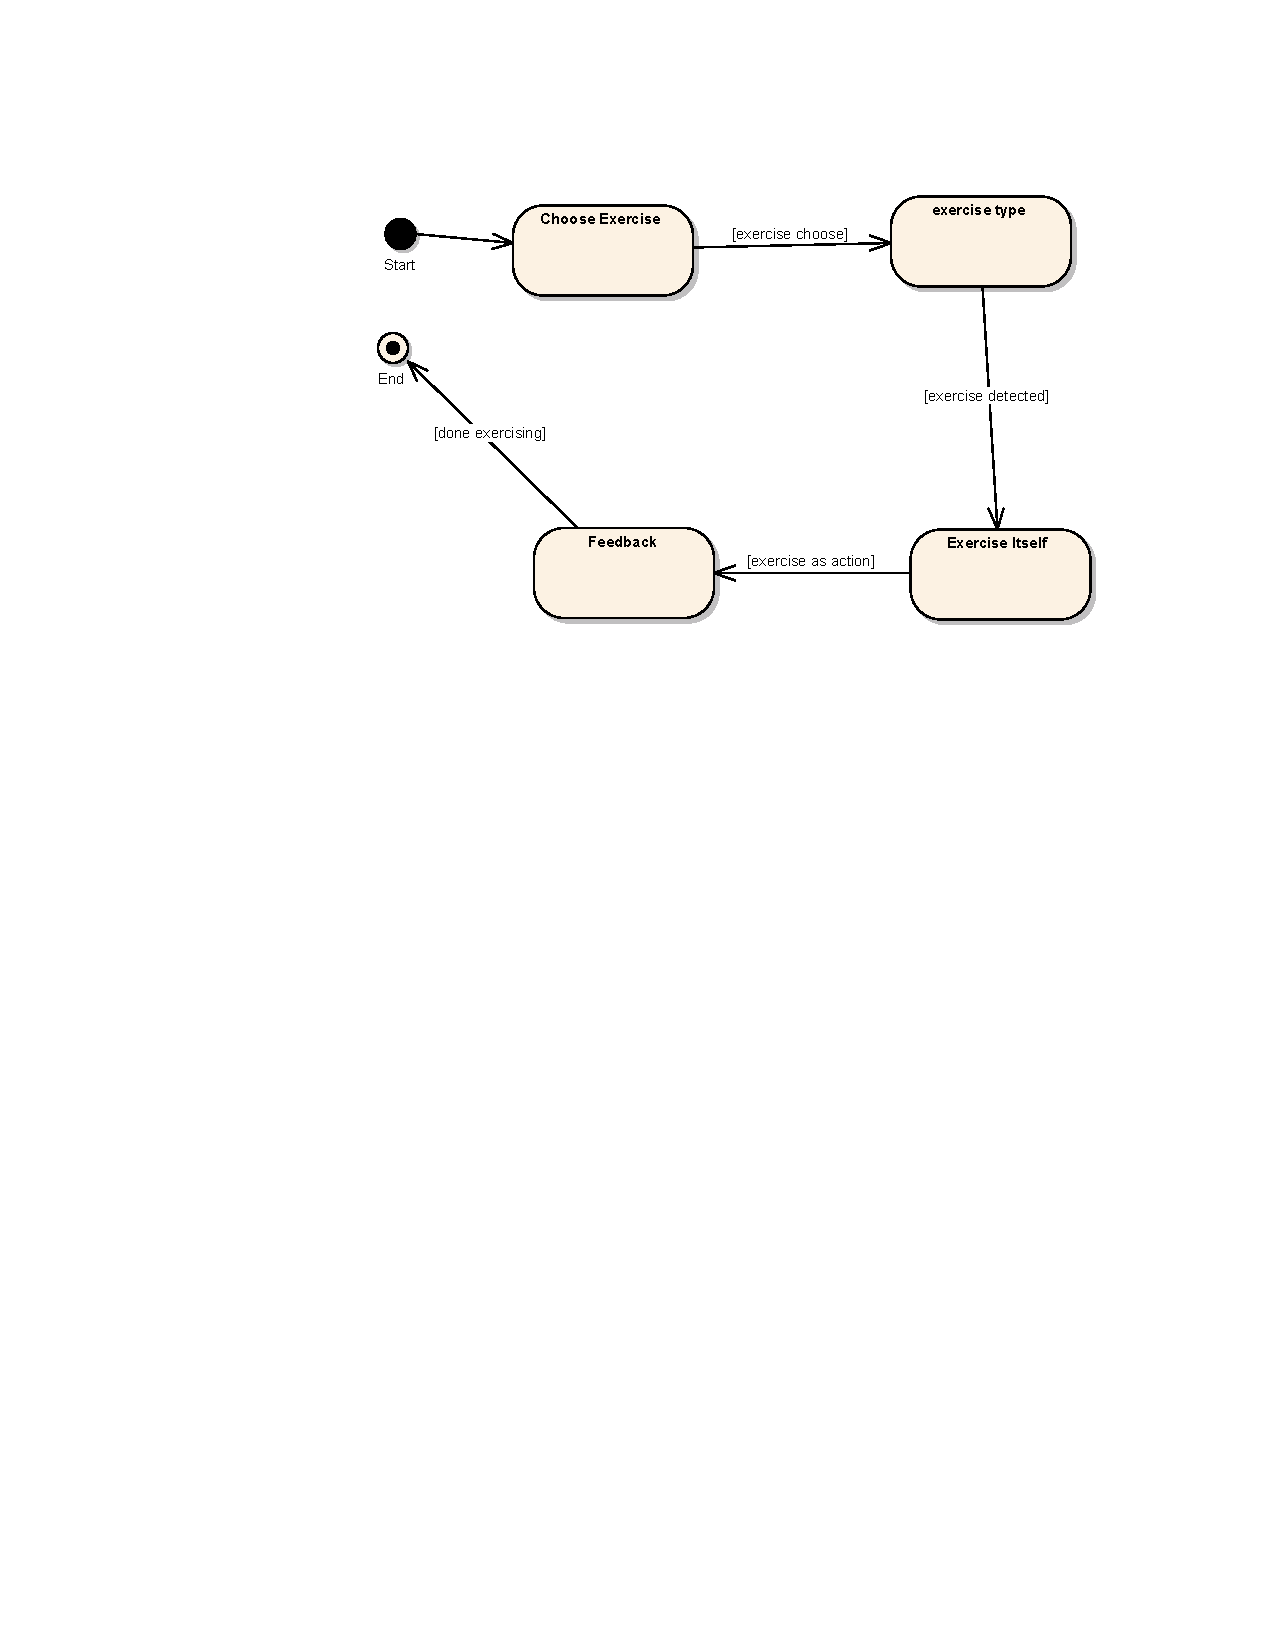
\includegraphics[trim={0 17cm 0 3cm},clip, width = 16cm]{2_state_performexercise}
\caption{State Diagram of exercising step by step.}\label{state_perform}
\end{figure}

\clearpage

\subsection{User Experience}


\clearpage